\documentclass[a4paper,12pt]{article}
\usepackage{graphicx}
\usepackage{bm,amssymb}
\usepackage{mathrsfs}
\usepackage[unicode,colorlinks=true,filecolor=blue, menucolor=black, linkcolor=black, citecolor=black,pagebackref=white]{hyperref}
\usepackage[utf8]{inputenc}
\usepackage[russian]{babel}
\usepackage{amsmath}
\usepackage{feynmp}
\usepackage{caption}
\usepackage[left=2cm,right=2cm, top=2cm,bottom=2cm,bindingoffset=0cm]{geometry}
\begin{document}
\title{Семинар по теме: <<Обыкновенные дифференциальные уравнения>>}
\maketitle

\subsection*{Задача 1 (разложение в ряд)}

Часто решение линейного дифференциального уравнения можно найти в
виде разложения в ряд по степеням $x$. Проиллюстрируем это на примере.
Найдём решение дифференциального уравнения Бесселя
\[
y^{\prime\prime}(x)+\frac{1}{x}y^{\prime}(x)+y(x)=0
\]

\noindent
в виде разложения $y(x)=\sum_{k=0}^{\infty}a_{k}x^{k}$. Функцией Бесселя называется
такое решение, которое в нуле регулярно и $J_{0}(0)=1$.


\subsubsection*{Решение}

Подставля $y(x)$ в нужном виде в уравнение, мы получаем:
\[
\sum_{k=2}^{\infty}k(k-1)a_{k}x^{k-2}+\sum_{k=1}^{\infty}a_{k}kx^{k-2}+\sum_{k=0}^{\infty}a_{k}x^{k}=0
\]


\[
\sum_{k=2}^{\infty}(k^{2}a_{k}+a_{k-2})x^{k-2}=0
\]

\noindent
Приравнивая коэффициенты при различных степенях $x$ нулю, мы получаем
рекуррентное соотношение $a_{k}=-\frac{1}{k^{2}}a_{k-2}$. Поскольку $y(0)=1$, то $a_1=0$ (т.к. это коэффициент перед $\frac{1}{x}$). Кроме того, $a_0=1$.

\noindent
Из этого мы заключаем, что все нечётные члены равны нулю $a_{2k-1}\equiv0$;
а чётные равны:

\[
a_{2k}=\frac{-1}{(2k)^{2}}\cdot\frac{-1}{(2(k-1))^{2}}\cdot\dots\cdot\frac{-1}{2^{2}}\cdot(-1)=\frac{(-1)^{k}}{2^{2k}(k!)^{2}}
\]


\[
y(x)\equiv J_{0}(x)=\sum_{k=0}^{\infty}\frac{(-1)^{k}}{(k!)^{2}}\left(\frac{x}{2}\right)^{2k}
\]
\noindent
\textit{Здесь необходим комменарий. Уравнение Бесселя имеет второй порядок по производной. Это, точно также, как и для гармонического осциллятора, означает, что имеется два линейно независимых решения. С другой стороны, используя разложение в ряд мы однозначно (с точностью до домножения на произвольную постоянную) нашли только одно решение. Встает вопрос: куда делось еще одно решение? Ответ состоит в том, что другое решение (которое обычно обозначают $Y_0(x)$ и называют функцией Неймана) не раскладывается в ряд в окрестности $x=0$. Более точно, при малых $x$ $Y_0(x)\simeq \frac{2}{\pi}\ln x$. Мы же, в свое время, при нахождении решения требовали его регулярности.}

\subsection*{Задача 2 (математический маятник)}

Рассмотрим классическое дифференциальное уравнение движения математического
маятника ($\omega^{2}=\frac{g}{l}$):
\[
\ddot{\varphi}=-\omega^{2}\sin\varphi
\]

\noindent
Если из положения равновесия маятнику придать необходимую начальную
скорость, конечное положение маятника может оказаться точно перевёрнутым.
Найдём такое решение.


\subsubsection*{Решение}

Для такого уравнения можно записать некую сохраняющуюся величину $E[\varphi(t)]$
(так называемый ``первым интегралом''; он может зависеть как от
$\varphi$ в некий момент времени, так и от производных). Сохранение
этой величины означает, что для любого $\varphi\left(t\right)$ -
решения уравнения, будет выполнено $\frac{d}{dt}E[\varphi(t)]\equiv0$.
В данном случае, выражение для первого интеграла можно написать из
физических соображений --- известно, что для консервативных систем имеется
закон сохранения энергии; в нашем случае его можно записать как:
\[
E[\varphi(t)]=\frac{1}{2}\dot{\varphi}^{2}-\omega^{2}\cos\varphi
\]

\noindent
Действительно:
\[
\frac{d}{dt}E[\varphi(t)]=\ddot{\varphi}\dot{\varphi}+\omega^{2}\sin\varphi\dot{\varphi}=\dot{\varphi}(\ddot{\varphi}+\omega^{2}\sin\varphi)\equiv0
\]
\noindent
Заметим, что если имеют место колебания амплитуды $\phi_0$, то $E=-\omega^{2}\cos\varphi_{0}$.\\\\
При помощи первых интегралов можно понижать степень уравнения. Действительно,
если величина $E$ сохраняется, то мы можем просто записать уравнение
уже первого порядка, которое является уравнением с разделяющимися переменными. Кроме того, подставим значение энергии через амплитуду колебаний $\phi_0$.
\[
E=\frac{1}{2}\dot{\varphi}^{2}-\omega^{2}\cos\varphi
\]
\[
\frac{d\varphi}{\sqrt{2(\cos\varphi-\cos\varphi_0)}}=\omega dt
\]
\noindent
Вернемся к поиску решения $\varphi(t)$. Если теперь проинтегрировать полученное тождество и разрешить его,
выразив $\varphi(t)$, мы полностью решим задачу в общем виде. Однако,
в общем случае интеграл в левой части не выражается через элементарные
функции; для таких интегралов введен целый класс специальных функций,
называемые эллиптическими интегралами. 
\noindent
В случае малых $\varphi_0$ его можно взять приближённо, заменив $\cos\varphi\approx1-\frac{\varphi^{2}}{2}$;
полученный ответ будет ни чем иным как гармоническим решением $\sin(\omega t+\varphi_{0})$.\\\\
С другой стороны, есть ещё один специальный случай, когда это уравнение 
можно решить точно --- случай $\varphi_0 = \pi$. При этом мы получаем:
\[
\int\frac{d\varphi}{\sqrt{2\omega^{2}(1+\cos\varphi)}}=t-t_{0}\Leftrightarrow\int\frac{d\varphi}{2\cos\frac{\varphi}{2}}=\omega(t-t_{0})
\]

\noindent
Интеграл берётся:
\[
\int\frac{d\varphi}{2\cos\frac{\varphi}{2}}=\int\frac{d(\sin\frac{\varphi}{2})}{1-\sin^{2}\frac{\varphi}{2}}=\left|\begin{array}{c}
\sin\frac{\varphi}{2}=\tanh z\\
d(\sin\frac{\varphi}{2})=\frac{dz}{\cosh^{2}z}
\end{array}\right|=\int dz=z={\rm arctanh}\sin\frac{\varphi}{2}
\]

\noindent
Тем самым, выражая $\varphi(t)$:
\[
\varphi(t)=2\arcsin\tanh\omega(t-t_{0})
\]


\begin{figure}[h]
\caption{Решение $\varphi(t)$}
\centering
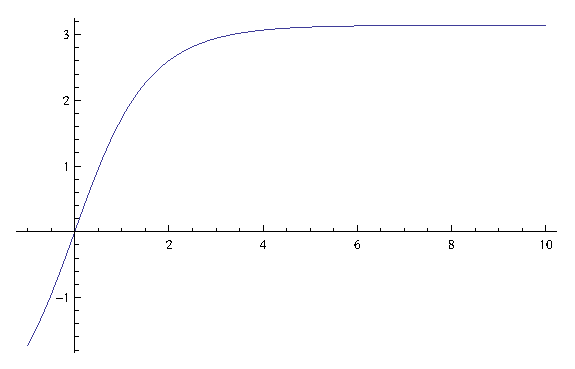
\includegraphics[width=0.5\columnwidth]{pendulum.eps}
\end{figure}
\noindent
Заметим, что для того, чтобы маятнику ``добраться'' до точки $\varphi=\pi$,
ему требуется бесконечное время (он лишь асимптотически приближается
к этому значению). В обратную сторону это означает, что из вертикального
положения маятник будет падать вечно; что, конечно, соответствует тому факту,
что $\varphi=\pi$ --- тоже положение равновесия системы.

\subsection*{Задача 3}

Воспользуемся аппаратом матричных экспонент для того, чтобы решить следующую систему дифференциальных уравнений
\[
\frac{d}{dt}
\begin{pmatrix}
x\\
y
\end{pmatrix}
=
A
\begin{pmatrix}
x\\
y
\end{pmatrix}
,\quad A=\begin{pmatrix}
-1 & 2\\
-3 & 4
\end{pmatrix}
\]
с начальным условием
\[
\begin{pmatrix}
x(0)\\
y(0)
\end{pmatrix}=
\begin{pmatrix}
1\\
0
\end{pmatrix}
\] 
\noindent


\subsubsection*{Решение}
В соответствии с материалом лекции, решение задачи выражается через
матричную экспоненту следующий образом
\[
\begin{pmatrix}
x(t)\\
y(t)
\end{pmatrix}
=
e^{At}
\begin{pmatrix}
x(0)\\
y(0)
\end{pmatrix}
\]
Для того, чтобы вычислить матричную экспоненту, необходимо диагонализовать матрицу $A$. Первый шаг в этой процедуре --- нахождение собственных значений при помощи секулярного уравнения
\[
\det (A-\lambda)=\det \begin{pmatrix}
-1-\lambda & 2\\
-3 & 4-\lambda
\end{pmatrix}=0\quad \rightarrow \quad \lambda_1=1,\quad \lambda_2=2
\]
Следующий шаг --- нахождение собственных векторов. Для этого необходимо решить систему линейных уравнений
\[
\begin{pmatrix}
-1-\lambda_{1/2} & 2\\
-3 & 4-\lambda_{1/2}
\end{pmatrix} h_{1/2}=0\quad \rightarrow \quad 
h_1=
\begin{pmatrix}
1\\
1
\end{pmatrix}
,\quad
h_2=
\begin{pmatrix}
2\\
3
\end{pmatrix}
\]
Тогда матрица перехода к диагональному базису записывается как
\[
S=
\begin{pmatrix}
h_1 & h_2
\end{pmatrix}
=
\begin{pmatrix}
1 & 2\\
1 & 3
\end{pmatrix}
\]
Для матричной экспоненты получаем
\[
e^{At}=Se^{A_\lambda}S^{-1},\quad A_\lambda = 
\begin{pmatrix}
1&0\\
0&2
\end{pmatrix}
\]
Вычисляя матрицу, обратную к матрице перехода, приходим к следующему выражению
\[
e^{At}=
\begin{pmatrix}
1&2\\
1&3
\end{pmatrix}
\begin{pmatrix}
e^t&0\\
0&e^{2t}
\end{pmatrix}
\begin{pmatrix}
3&-2\\
-1&1
\end{pmatrix}
=
\begin{pmatrix}
3e^t-2e^{2t}&-2e^t+2e^{2t}\\
3e^t-3e^{2t}&-2e^t+3e^{2t}
\end{pmatrix}
\]
Стало быть, решение задачи с данным начальным условием $x(0)=1$, $y(0)=0$ дается следующим выражением
\[
\begin{pmatrix}
x(t)\\
y(t)
\end{pmatrix}
=
\begin{pmatrix}
3e^t-2e^{2t}\\
3e^t-3e^{2t}
\end{pmatrix}
\]
\subsection*{Приложение: матричная экспонента от Жордановой клетки}
Стоит иметь в виду, что \textit{не любую} матрицу можно диагонализовать. При этом, согласно теореме Жордана, совершенно \textit{любую} матрицу можно привести к Жордановому виду --- блок-диагональной форме, в которой каждый блок представляет собой сумму $\lambda E + M$, где $\lambda$ - некоторое число, $E$ - единичная матрица, а $M$ - матрица вида
\[
M=
\begin{pmatrix}
0 & 1 & 0 & ... & 0 & 0\\
0 & 0 & 1 & ... & 0 & 0\\
... &  &  &  &  & ...\\
0 & 0 & 0 & ... & 0 & 1\\
0 & 0 & 0 & ... & 0 & 0\\
\end{pmatrix}
\]
Комбинация $\lambda E + M$ называется Жордановой клеткой.
Возникает уместный вопрос: как вычислять матричную экспоненту для такой Жордановой клетки?\\\\
Не углубляясь в детали, рассматотрим пример взятия матричной экспоненты от Жордановой матрицы размера $2\times2$. Таким образом, мы изучаем матрицу
\begin{equation}
A=\left(\begin{array}{cc}
\lambda & 1\\
0 & \lambda
\end{array}\right)
\notag
\end{equation}
Разобьем ее

\[
A=\lambda E+M,\quad\quad\quad M=\left(\begin{array}{cc}
0 & 1\\
0 & 0
\end{array}\right)
\]
Заметим, что

\[
M^{2}=0,
\]
а тогда равны нулю и все степени M, кроме нулевой и первой. Это соображение позволяет нам очень легко вычислить произвольную степень $n$ матрицы $A$, использую бином Ньютона

\begin{equation}
A^{n}=\lambda^{n}E+n\lambda^{n-1}M
\notag
\end{equation}
Видим, что

\[
e^{tA}=e^{\lambda t}+\sum_{n=1}^{\infty}n\lambda^{n-1}\frac{t^{n}}{n!}M=e^{\lambda t}+M\frac{\partial}{\partial\lambda}\sum_{n=0}^{\infty}\lambda^{n}\frac{t^{n}}{n!}=e^{\lambda t}+M\frac{\partial}{\partial\lambda}e^{\lambda t}=e^{\lambda t}(E+tM)
\]
Иными словами,

\begin{equation}
e^{tA}=\left(\begin{array}{cc}
1 & t\\
0 & 1
\end{array}\right)e^{\lambda t}
\notag
\end{equation}
В заключение отметим, что для Жордановых клеток размера, больше чем $2 \times 2$, помимо линейных по $t$ элементов, могут появиться элементы с высшими степенями $t$.

\subsection*{Задачи для домашнего решения}

\noindent \textbf{Упражнение 1}

\noindent Движение маятника в нелинейном пределе описываяется следующим уравнением:
\begin{equation}\notag
\frac{d\phi}{dt}=\pm\omega\sqrt{2(\cos\phi-\cos\phi_{0})},
\end{equation}
где $\phi_{0}$ - его максимальное отклонение от положения равновесия в процессе движения. Пусть в начальный момент он практически перевернут, то есть $\phi(0)=\phi_{0}=\pi-\delta\phi$, $\dot{\phi}(0)=0$, где $\delta\phi\ll 1$. Оцените время падения маятника до положения $\phi=0$.

\vspace{15pt}
\noindent \textbf{Упражнение 2}

\noindent Используя матричную экспоненту, решите систему дифференциальных уравнений
\begin{equation}\notag
\left(\begin{array}{c}
\dot{x}(t)\\
\dot{y}(t)
\end{array}\right)	=\left(\begin{array}{cc}
2 & 1\\
4 & 5
\end{array}\right)\left(\begin{array}{c}
x(t)\\
y(t)
\end{array}\right),\quad\left(\begin{array}{c}
x(0)\\
y(0)
\end{array}\right)=\left(\begin{array}{c}
1\\
0
\end{array}\right).
\end{equation}

\vspace{15pt}
\noindent \textbf{Упражнение 3}

\noindent Найдите разложение в ряд по $x$ функции Бесселя $J_{m}(x)$ целого порядка $m$, определяемой как решение дифференциального уравнения:
$$
y^{\prime\prime}(x)+\frac{1}{x}y^{\prime}(x)+\left(1-\frac{m^2}{x^2}\right)y(x)=0
$$

\vspace{15pt}
\noindent \textbf{Упражнение 4}

\noindent Найдите общее решение уравнения движения маятника с вязким трением:

\begin{equation}
\notag
\ddot{x}(t)+2\gamma \dot{x}(t) +\omega^2 x(t)=0.
\end{equation} 

\noindent Качественно проанализируйте различные режимы движения в зависимости от соотношения между $\gamma$ и $\omega$.

\vspace{15pt}
\noindent \textbf{Задача 1}

\noindent В сверхпроводнике электроны ведут себя принципиально отлично от электроннов в обычном металле. В определенном смысле, они движутся парами (такие пары называются куперовскими). Для макроскопическом описания такого поведения вводят функцию $\psi$, которая в каждой точке пропорциональна $\sqrt{n}$, где $n$ - плотность куперовских пар, а в толще сверхпроводника равна $1$\text{.}

\noindent Уравнение, которое описывает поведение функции $\psi$ называется уравнением Гинзбурга-Ландау. В простейшем случае, оно имеет вид
\begin{equation}\notag
-\xi^{2}\frac{d^{2}\psi}{dx^{2}}-\psi+\psi^{3}	=0,
\end{equation}
\noindentгде $\xi$ - некоторая величина размерности расстояния.

\noindentПрименим его, чтобы описать контакт сверхпроводника с обычным металлом. \noindentПусть полупространство $x>0$ занимает сверхпроводник, а полупространство $x<0$ - нормальный металл. Для простоты будем считать, что куперовские пары совсем не проникают в металл, то есть $\psi(0)=0$. Учитывая, что $\psi(+\infty)=1$, найдите $\psi(x)$.

\vspace{15pt}
\noindent \textbf{Задача 2}

\noindent Введем набор из трех эрмитовых матриц размера $2$ на $2$, которые называются матрицами Паули:
\begin{equation}\notag
\sigma_{x}=\left(\begin{array}{cc}
0 & 1\\
1 & 0
\end{array}\right),\quad\sigma_{y}=\left(\begin{array}{cc}
0 & -i\\
i & 0
\end{array}\right),\quad\sigma_{z}=\left(\begin{array}{cc}
1 & 0\\
0 & -1
\end{array}\right).
\end{equation}

\noindent Можно определить скалярное произведение произвольного вектора $\vec{a}=(a_{x},a_{y},a_{z})^{T}$ на вектор из матриц Паули $\vec{\sigma}=(\sigma_{x},\sigma_{y},\sigma_{z})^{T}$ стандартным образом: $\left(\vec{a}\cdot\vec{\sigma}\right)=\sum_{i=x,y,z}a_{i}\sigma_{i}$.

\noindent Вычислите следующую матричную экспоненту
\begin{equation}\notag
e^{i\tau\left(\vec{n}\cdot\vec{\sigma}\right)},
\end{equation}
\noindent где $\vec{n}$ - единичный вектор с произвольным направлением, а $\tau$ - произвольное действительное число.

\noindent \textit{Примечание: выражение такого типа естественным образом возникает в квантовой механике при описании движения магнитного момента электрона в магнитном поле. В этом случае вектор $\vec{n}$ задает направление поля $\vec{B}$, а $\tau\sim Bt$, где $t$ - время.}
\end{document}
